\documentclass[a4paper]{article}
\usepackage{ulem}
\usepackage{graphicx}
\usepackage[namelimits]{amsmath}
\usepackage{amssymb}
\usepackage{amsmath}
\usepackage{amsfonts}
\usepackage{mathrsfs}
\usepackage{enumerate}
\usepackage{indentfirst}
\usepackage{multirow}
\usepackage{latexsym}
\usepackage{subfig}
\usepackage{listings}
\usepackage{xcolor}

\lstset{numbers=left,
	numberstyle=\tiny,
	frame=shadowbox,
	backgroundcolor=\color[RGB]{245,245,244},
	keywordstyle=\color[RGB]{40,40,255},
	numberstyle=\footnotesize\color{darkgray},
	commentstyle=\color[RGB]{50,50,50},
	breaklines=true,
	tabsize=4,
	showspaces=false}

\title{UM-SJTU JOINT INSTITUTE\\VE482 Introduction to Operating Systems\\\vspace{0.5cm} Homework 2}
\author{Li Yong 517370910222}
\begin{document}
\maketitle
\newpage

\section*{Ex.1 Multiprogramming}
	\begin{enumerate}
		\item $P[$process to be waiting$] = p$\\
		$P[n$ processes to be waiting$] = p^n$\\
		utilisation$(n) = 1-p^n$
		\item Plot by \textit{Mathematica}
		\begin{figure}[ht]
			\centering
			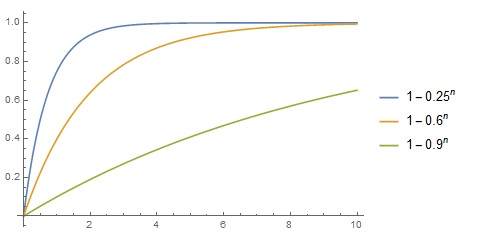
\includegraphics[scale=0.7]{utilisation.png}
		\end{figure}
		\item
		\begin{enumerate}[a)]
			\item $$(256-96)/48=3.33$$
			Hence 3 processes can be store simultaneously in memory.
			\item $$1-0.9^3=0.271$$
			\item Adding 256MB:
			$$(256+256-96)/48=8.67$$
			$$1-0.9^8=0.5695$$
			$$0.2848/256MB$$
			Adding 512MB:
			$$(256+512-96)/48=14$$
			$$1-0.9^{14}=0.7712$$
			$$0.2571/256MB$$
			Adding 1024MB:
			$$(256+1024-96)/48=24.67$$
			$$1-0.9^{24}=0.9202$$
			$$0.1840/256MB$$
			Hence, adding 256MB is the most beneficial and would be worth the investment.
		\end{enumerate}
	\end{enumerate}

\section*{Keymap in Minix 3}
	\begin{enumerate}
		\item Add the keymap in \texttt{/usr/src/servers/is/dmp.c}
		\begin{lstlisting}[language=C]
struct hook_entry {
	int key;
	void (*function)(void);
	char *name;
} hooks[] = {
	{ F1, proctab_dmp, "Kernel process table" },
	{ F3,	image_dmp, "System image" },
	{ F4,	privileges_dmp, "Process privileges" },
	{ F5,	monparams_dmp, "Boot monitor parameters" },
	{ F6,	irqtab_dmp, "IRQ hooks and policies" },
	{ F7,	kmessages_dmp, "Kernel messages" },
	{ F8,	vm_dmp, "VM status and process maps" },
	{ F10, kenv_dmp, "Kernel parameters" },
	{ SF1, mproc_dmp, "Process manager process table" },
	{ SF2, sigaction_dmp, "Signals" },
	{ SF3, fproc_dmp, "Filesystem process table" },
	{ SF4, dtab_dmp, "Device/Driver mapping" },
	{ SF5, mapping_dmp, "Print key mappings" },
	{ SF6, rproc_dmp, "Reincarnation server process table" },
	//Shift+F7 keymap
	{ SF7, procnum_dmp, "Print the number of currently running process"},
	{ SF8, data_store_dmp, "Data store contents" },
	{ SF9, procstack_dmp, "Processes with stack traces" },
};
		\end{lstlisting}
		\item Declare the function \texttt{procnum\_dmp()} in \texttt{/usr/src/servers/is/proto.h}
		\begin{lstlisting}[language=C]
void procnum_dmp(void);
		\end{lstlisting}
		\item Implement \texttt{procnum\_dmp()} in \texttt{/usr/src/servers/is/dmp\_kernel.c}
		\begin{lstlisting}[language=C]
/*===========================================*
*				procnum_dmp				     *
*============================================*/
void procnum_dmp()
{
   struct proc *runningProc;
   int procNum = 0;
   int r;
   if ((r = sys_getproctab(proc)) != OK)
   {
       printf("IS: warning: couldn't get copy of process table: %d\n", r);
  	   return;
   }
   for (runningProc = BEG_PROC_ADDR; runningProc < END_PROC_ADDR; runningProc++)
   {
       if (!isemptyp(runningProc))
       {
           procNum++;
       }
   }
   printf("The number of currently running process: %d\n", procNum);
}
		\end{lstlisting}
		\item Rebuild
		\begin{lstlisting}[language=bash]
cd /usr/src/releasetools
make hdboot
		\end{lstlisting}
		\item Demo
		\begin{figure}[ht]
			\centering
			
\includegraphics[scale=0.7]{demo.png}
		\end{figure}
	\end{enumerate}
\end{document}
